\chapter{Übersicht der Hardwarekomponenten}
\label{c:hardware}
\section{Komponentenbeschreibung}
Im Folgenden soll eine Übersicht aller Hardwarekomponenten erfolgen. Dadurch
soll eine grobe Vorstellung der Funktionsweise des Mikrorechners entstehen,
welche in Kapitel~\ref{c:vhdl} vertieft wird. Vor der Beschreibung der einzelnen
Hardwarekomponenten soll durch Abbildung~\ref{pic:hardware_overview} das
Zusammenspiel aller Komponenten gezeigt werden, auf welche während dieses
Kapitels zurückgegriffen werden kann.
\begin{figure}[hb]
\centering
\def\svgwidth{\columnwidth}
\input{img/hardware_overview.pdf_tex}
\caption{Hardwarekomponentenübersicht}
\label{pic:hardware_overview}
\end{figure}
\pagebreak
\subsection{Steuerwerk}
\label{s:control}
Das Steuerwerk ist dafür zuständig, die einzelnen Zustände, die bei der
Ausführung jedes Befehls ausgeführt werden, zum richtigen Zeitpunkt zu
aktivieren. Dabei können einzelne Zustände je nach Befehl übersprungen werden.

Als Abstraktion kann man sich das Steuerwerk auch als Zustandsautomat
vorstellen. Mit Hilfe von Abbildung~\ref{pic:zustandsdiagramm} soll die
Funktionsweise des Steuerwerkes durch ein Zustandsdiagramm dargestellt werden.

\begin{figure}[htb]
\centering
\begin{tikzpicture}[->,>=stealth',shorten >=1pt,auto,node distance=4cm,
					semithick]

	\tikzstyle{every state}=[fill=white,draw=black,text=black,minimum size=6em]

	\node[initial,state]	(A)						{Fetch};
	\node[state]			(B) [above right of=A]	{Decode};
	\node[state]			(C) [right of=B]		{Read};
	\node[state]			(D) [below of=C]		{Execute};
	\node[state]			(F) [below of=D]		{Stack R/W};
	\node[state]			(E) [right of=F]		{Memory Write};
	\node[state]			(G) [left of=F]			{Reg Write};

	\path	(A) edge					node {} (B)
			(B) edge					node {} (C)
			(C) edge 					node {} (D)
			(D) edge 					node {} (E)
				edge 					node {} (F)
				edge 					node {} (G)
			(E) edge [bend left=100]	node {} (A)
			(F) edge [bend left=100]	node {} (A)
				edge					node {} (G)
			(G) edge 					node {} (A);

\end{tikzpicture}
\caption{Zustandsdiagramm des Steuerwerks}
\label{pic:zustandsdiagramm}
\end{figure}
\pagebreak
Die einzelnen Zustände des Steuerwerks werden im Folgenden beschrieben.
\subsubsection{Fetch}
Der zunächst auszuführende Befehl wird aus dem Hauptspeicher in den Prozessor
geladen. Die Adresse des Befehls wird durch den Wert des Programmzählers
(siehe~\ref{s:stack}) bestimmt.
\subsubsection{Decode}
In diesem Zustand wird das erste Byte des Befehl dekodiert und dabei
festgestellt, ob der Befehl noch mehr Bytes, als bisher gelesen wurde, besitzt.
Ist dies der Fall, wird wieder zum "`Fetch"'-Zustand gewechselt. Außerdem wird der
eigentlich auszuführende Befehl festgestellt, mit welchen Parametern er
auszuführen ist, aus welchen Registern die Daten kommen und wo das Resultat
gespeichert werden soll. Eine ausführlichere Beschreibung ist bei der
Beschreibung des Dekodiers in Abschnitt~\ref{s:decode} zu finden.
\subsubsection{Read}
Die Register für die Ein- und Ausgabe des Befehls werden nun ausgewählt und
dementsprechend ist genug Zeit vorhanden, die Daten zu lesen, sodass keine
korrupte Daten in den folgenden Zuständen zur Verwendung kommen.
\subsubsection{Execute}
Das Rechenwerk (siehe~\ref{s:alu}) wird bei diesem Zustand aktiviert und führt
den vorher dekodierten Befehl aus. Das Resultat des Rechenwerks wird ausgegeben,
damit in den weiteren Zuständen das Ergebnis an die gewünschte Stelle
geschrieben werden kann.
\subsubsection{Memory Write}
Das Resultat des Rechenwerks wird an die vom Befehl vorgebene Speicheradresse im
Arbeitsspeicher (siehe~\ref{s:memorycontrol}) gespeichert.
\subsubsection{Stack Read/Write}
Je nach Befehl wird entweder das Resultat des Rechenwerks auf dem Stack gelegt
oder der oberste Wert des Stacks genommen, um es im nächsten Zustand weiter
verarbeiten zu können. Eine detaillierte Erklärung der Funktionsweise des Stacks
findet in Abschnitt~\ref{s:stack} statt.
\subsubsection{Register Write}
Ähnlich wie beim "`Stack Read/Write"'-Zustand, wird auch hier (je nach Befehl) das
Ergebnis des Rechenwerks oder der Wert, der vom Stack entnommen wurde, in das
Register geschrieben, welches der Befehl vorschreibt.
\subsection{Rechenwerk}
\label{s:alu}
Das Rechenwerk ist dafür zuständig, dass die eigentliche Operation des Befehls
ausgeführt wird. Es ist zu unterscheiden, ob man von der \ac{ALU} oder vom
Rechenwerk spricht, denn die \ac{ALU} ist nur das "`Rechenzentrum"' des
Rechenwerks, gestützt von z.B. Hilfsregistern.

Der Befehlscode (auch Opcode) besteht aus 5 Bits und daher können $2^{5} = 32$
verschiedene Befehle ausgeführt werden. Mit Hilfe der
Tabelle~\ref{tab:befehlsliste} soll ein Überblick über die verfügbaren Befehle
vermittelt werden. Um den Aufbau simpel zu halten, wurde entschieden, dass jeder
Befehl die gleiche Bearbeitungszeit bekommt und damit jeder Befehl gleich
schnell (bezogen nur auf die Zeit beim Rechenwerk) ausgeführt wird.

Das Rechenwerk hat die Aufgabe bestimmte Statusflaggen zu setzen oder zu
löschen. Im Beispiel "`SB"' gibt die Statusflagge an, ob ein Sprungbefehl
ausgeführt wird und dieser auch die Sprungbedingung erfüllt. Der Programmzähler
erhält in diesem Fall einen neuen Wert.
\clearpage
\pagebreak
\subsection{Dekodierer}
\label{s:decode}
Der Dekodierer übernimmt die Aufgabe, den Befehl zu dekodieren, damit die
Operation für das Rechenwerk ausgewählt werden kann und die dafür benötigten
Register angesprochen werden. Da der Dekodierer einen einfachen Aufbau haben
sollte, wurde der Aufbau eines Befehls selbst einfach gehalten.

Der Dekodierer ist sehr stark an den Befehlssatz angelehnt, welcher in
Abschnitt~\ref{s:befehlssatz} genauer beschrieben wird.
\subsection{Programmzähler}
\label{s:pc}
Der Programmzähler (engl. \ac{PC}) ist hardwaretechnisch gesehen ein Register,
welches aber im Vergleich zu "`normalen"' Registern ihren Wert um eine bestimmte
Byteanzahl (je nach Länge des ausgeführten Befehls) erhöht. Somit hält der \ac{PC}
immer die Adresse für den nächsten auszuführenden Befehl. Bei einem Sprungbefehl
wird der Wert des Programmzählers mit dem vom Befehl vorgeschriebenen Wert
überschrieben.

Im Ganzen lässt sich der Programmzähler als Zustandsautomat realisieren. Dazu
wurden vier verschiedene Zustände für den \ac{PC} gewählt:

\begin{labeling}{\textbf{ASSIGN}}
\item[\textbf{NOP}]		Keine Operation
\item[\textbf{INC}]		Erhöhe den Zähler um die Byteanzahl des vorherigen Befehls
\item[\textbf{ASSIGN}]	Setze den Zähler auf die Sprungadresse
\item[\textbf{RESET}]	Setze den Zähler auf null zurück
\end{labeling}

Je nach Befehl wird bei der Ausführung dann der passende Zustand ausgewählt und
somit sichergestellt, dass die Adresse für den folgenden Befehl korrekt ist.
\subsection{Stack}
\label{s:stack}
Der Stack (deutsch: Stapel) ist ein Modell zum Speichern von Daten. Dabei sind
zwei Operationen zum Speichern und Abrufen der Daten vorhanden: PUSH und POP\@.
Bei PUSH wird oben auf den Stapel ein neues Element hinzugefügt, bei POP wird
das oberste Element vom Stapel heruntergenommen. Somit ist der Zugriff auf das
oberste Element beschränkt. Der Stack wird hauptsächlich von Programmen als
Zwischenspeicher genutzt, wenn nicht genügend Register zur Verfügung stehen,
aber auch beim Aufrufen von Funktionen (Befehl CALL) wird auf dem Stack die
Rückkehraddresse gespeichert, welche beim Verlassen der Funktion (Befehl RET)
wieder vom Stapel entnommen wird.

Besonders für den Funktionsaufruf eignet sich das Prinzip des Stacks sehr gut,
da es keine Limitierung der Anzahl der Funktionsaufrufe gibt (außer der
physikalischen Größe des Stacks). Somit ist es möglich, dass unbegrenzt viele
Funktionen ineinander aufgerufen werden können. Es sind also theoretisch
unendlich viele Verkettungen möglich, wobei die Theorie nur durch die maximale
Größe des Stacks limitiert wird.

\subsection{UART}
\label{s:uart}
Der \ac{UART}, welcher die Implementierung der seriellen Schnittstelle enthält,
wird genutzt, um Eingabe von dem Benutzer zu bekommen. Dabei wird über ein
selbst geschriebenes Skript die Tastatureingabe von einem anderen Rechner
übernommen und über die serielle Schnittstelle an das Gerät weitergeleitet. So
ist es möglich, eine Tastatur "`anzuschließen"'. Die Übertragung über die serielle
Schnittstelle findet mit einer Bitrate von 9600 bit/s, 8 Datenbits, 1 Stopbit
und keinem Paritätsbit statt.

Hardwaretechnisch ist der UART über die Speicheradresse 0xEF00 zu erreichen.
Sollte diese Adresse gelesen werden, wird das nächste Byte des UARTs abgefragt
und dadurch die CPU temporär gestoppt, bis ein Byte angekommen ist. Dadurch ist
die Eingabe blockierend, es können also keine weiteren Operationen während der
Eingabe durchgeführt werden.
\subsection{Speichercontroller}
\label{s:memorycontrol}
Der Arbeitsspeicher ist als kontinuierlicher Speicherblock realisiert worden. Es
sind zwei Ports für die Ein- und Ausgabe zur Verfügung, wobei der zweite Port
ausschließlich für den Videocontroller vorgesehen ist, welcher damit Zugriff auf
den Videospeicher bekommt. Dies bedeutet auch, dass der Videospeicher nicht
separat geändert werden muss und so über allgemein gültige Lese- und
Schreibbefehle angesprochen werden kann.

Insgesamt wurde der mit 16 Bit verfügbare maximal adressierbare Speicher von
$2^{16} = 65536$ Bytes ausgenutzt, wobei einzelne Abschnitte, wie beispielsweise
der Videospeicher oder auch die Speicheraddresse für den UART nicht allgemein nutzbar sind.
\subsection{Videocontroller}
\label{s:videocontrol}
Der Videocontroller selbst ist nach außen hin unabhängig von allen anderen
Elementen der \ac{EPU}. Nur der Videospeicher, welche die Informationen über die
anzuzeigenden Pixel enthält, wird vom Speichercontroller geliefert. Dennoch hat
der Speichercontroller keine Kontrolle über den Zugang des Videcontrollers zu
dem Videospeicher, denn wie bereits in~\ref{s:memorycontrol} beschrieben, ist der
Port für den Videocontroller unabhängig vom Speichercontroller.
\pagebreak
\subsection{Registerbelegung}
Die \ac{EPU} besitzt 16 Register, welche durch Selektion von $\log_2(16) = 4$
Adressbits angesprochen werden. Mithilfe der Tabelle~\ref{tab:registerbelegung}
soll eine Übersicht aller Register dargestellt werden.

\begin{table}[h]
\centering
\begin{tabular}{lll}
\toprule
Selektion & Name & Zweck\\
\midrule
0000 & R0  & Akkumulator\\
0001 & R1  & Allgemeine Verwendung\\
0010 & R2  & Allgemeine Verwendung\\
0011 & R3  & Allgemeine Verwendung\\
0100 & R4  & Allgemeine Verwendung\\
0101 & R5  & Allgemeine Verwendung\\
0110 & R6  & Allgemeine Verwendung\\
0111 & R7  & Allgemeine Verwendung\\
1000 & R8  & Allgemeine Verwendung\\
1001 & R9  & Allgemeine Verwendung\\
1010 & R10 & Allgemeine Verwendung\\
1011 & R11 & Allgemeine Verwendung\\
1100 & R12 & Allgemeine Verwendung\\
1101 & R13 & Allgemeine Verwendung\\
1110 & R14 & Flagregister\\
1111 & R15 & Programmzähler (Kopie)\\
\bottomrule
\end{tabular}
\caption{Registerbelegung}
\label{tab:registerbelegung}
\end{table}
\pagebreak
\section{Befehlssatz}
\label{s:befehlssatz}
Der Befehlssatz beschreibt den Aufbau und die Menge aller Befehle der \ac{EPU}.
Nachfolgend soll sowohl der Aufbau sowie dessen Entstehung erläutert werden.

\subsection{Aufbau}
Der Befehl wird byteweise gelesen. Die Anzahl an Bytes in einem Befehl sind
durch die beiden letzten Bits des ersten Bytes angegeben, was es leichter macht,
die richtige Byteanzahl einzulesen. Alle weiteren Abschnitte jedes Bytes werden
je nach Opcode (die ersten 5 Bits) bestimmt, also die Register, die
Rechenoperation, ob das Ergebnis auf dem Arbeitsspeicher geschrieben werden
soll etc. Wie in Abbildung~\ref{pic:befehlsaufbau} zu sehen, ist die Angabe
von Konstanten in 4, 8 und 16 Bit möglich. Der Grund für die doch sehr
platznehmende 16-Bit-Konstante ist, dass ein Register mit einer Konstante in
einem Befehl befüllt werden soll, wobei alle Register der \ac{EPU} 16 Bit groß
sind.
\begin{figure}[htb]
\centering
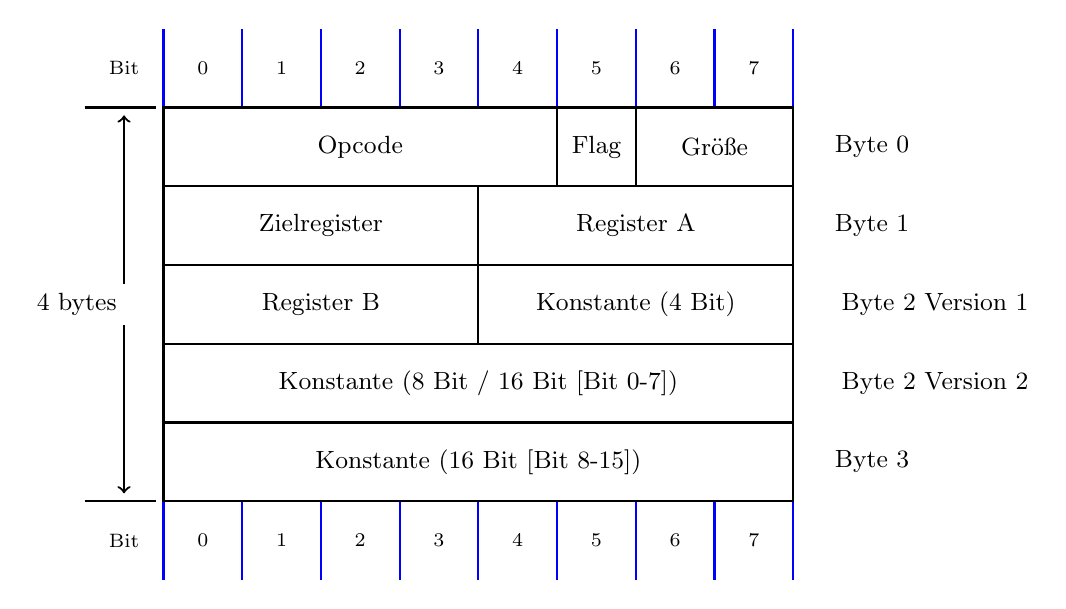
\begin{tikzpicture}
	% Bitnummern oben
	\foreach \x in {0,...,7}
		\node at (\x + 0.5, 20.5) {\scriptsize \x};
	% Bitnummern unten
	\foreach \x in {0,...,7}
		\node at (\x + 0.5, 14.5) {\scriptsize \x};
	% Blaue vertikale Linien
	\foreach \x in {0,...,8}
		\draw[thick,blue] (\x, 14) -- (\x,21);
	% Das Wort ""'Bit""' nach ganz links schreiben
	\node[thick] (bit1) at (-0.5, 20.5) {\scriptsize Bit};
	\node[thick] (bit2) at (-0.5, 14.5) {\scriptsize Bit};
	% Pfeil links
	\draw[<->, thick] (-0.5, 19.9) -- (-0.5, 15.1);
	\draw[thick] (-1, 20) -- (-0.1, 20);
	\draw[thick] (-1, 15) -- (-0.1, 15);
	\node[fill=white] at (-1.1, 17.5) {\small 4 bytes};
	% Byte 0
	\filldraw[thick, draw=black, fill={rgb:white,255}] (0, 20) rectangle (5, 19);
	\node (mode) at (2.5, 19.5) {\small Opcode};
	\filldraw[thick, draw=black, fill=white] (5, 20) rectangle (6, 19);
	\node (mode) at (5.5, 19.5) {\small Flag};
	\filldraw[thick, draw=black, fill=white] (6, 20) rectangle (8, 19);
	\node (mode) at (7, 19.5) {\small Größe};
	\node[fill=white] at (9, 19.5) {\small Byte 0};
	% Byte 1
	\filldraw[thick, draw=black, fill=white] (0, 19) rectangle (4, 18);
	\node (mode) at (2, 18.5) {\small Zielregister};
	\filldraw[thick, draw=black, fill=white] (4, 19) rectangle (8, 18);
	\node (mode) at (6, 18.5) {\small Register A};
	\node[fill=white] at (9, 18.5) {\small Byte 1};
	% Byte 2
	\filldraw[thick, draw=black, fill=white] (0, 18) rectangle (4, 17);
	\node (mode) at (2, 17.5) {\small Register B};
	\filldraw[thick, draw=black, fill=white] (4, 18) rectangle (8, 17);
	\node (mode) at (6, 17.5) {\small Konstante (4 Bit)};
	\node[fill=white] at (9.8, 17.5) {\small Byte 2 Version 1};
	% Byte 2 Alternative
	\filldraw[thick, draw=black, fill=white] (0, 17) rectangle (8, 16);
	\node (mode) at (4, 16.5) {\small Konstante (8 Bit / 16 Bit [Bit 0-7])};
	\node[fill=white] at (9.8, 16.5) {\small Byte 2 Version 2};
	% Byte 3
	\filldraw[thick, draw=black, fill=white] (0, 16) rectangle (8, 15);
	\node (mode) at (4, 15.5) {\small Konstante (16 Bit [Bit 8-15])};
	\node[fill=white] at (9, 15.5) {\small Byte 3};
\end{tikzpicture}
\caption{Befehlsaufbau}
\label{pic:befehlsaufbau}
\end{figure}
\subsection{Befehlsübersicht}
Die folgende Tabelle~\ref{tab:befehlsliste} soll einen Überblick über die
verschiedenen Befehle der \ac{EPU} liefern. Durch die Größe des Opcodes (5 Bit)
sind insgesamt $2^5 = 32$ Befehle möglich. Dennoch kann ein Befehl durch
bestimmte Parameter (wie z.B. der Flag im ersten Byte) um gewisse Funktionen
erweitert werden. Dies ermöglicht beispielsweise vorzeichenbehaftete und
vorzeichenlose Addition, obwohl der Opcode beider Operationen der Gleiche ist.
Eine ausführlichere Beschreibung jedes Befehls ist im
Anhang~\ref{a:befehlsliste} zu finden.
\begin{table}[htb]
\centering
\begin{tabular}{lll}
\toprule
Beschreibung									& Kurzform	& Opcode\\
\midrule
Keine Operation									& NOP		& 00000\\
Addition										& ADD   	& 00001\\
Subtraktion										& SUB   	& 00010\\
Logisches UND									& AND   	& 00011\\
Logisches ODER									& OR    	& 00100\\
Logisches XOR									& XOR   	& 00101\\
Logisches NOT									& NOT   	& 00110\\
Laden eines Registers							& LOAD  	& 00111\\
Verschieben eines Registerwertes				& MOV   	& 01000\\
Lesevorgang im Arbeitsspeicher					& READ  	& 01001\\
Schreibvorgang im Arbeitsspeicher				& WRITE 	& 01010\\
Bitweises Verschieben nach links				& SHL   	& 01011\\
Bitweises Verschieben nach rechts				& SHR   	& 01100\\
Vergleichen zweier Register						& CMP   	& 01101\\
Springen zu einer Adresse						& JMP   	& 01110\\
Bedingtes Springen zu einer Adresse				& JC    	& 01111\\
Nicht benutzt									& ---   	& 10000\\
Aufrufen einer Funktion							& CALL  	& 10001\\
Zurückkehren von einer Funktion					& RET   	& 10010\\
Ein Element auf den Stack schieben				& PUSH  	& 10011\\
Von dem Stack ein Element entnehmen				& POP   	& 10100\\
Nicht benutzt									& ---   	& 10101\\
Flags für die Beziehung zweier Register setzen	& TEST  	& 10110\\
Nicht benutzt									& ---   	& 10111\\
Nicht benutzt									& ---   	& 11000\\
Stoppen der Ausführung des Prozessors			& HLT   	& 11001\\
Setzen eines bestimmten Bits eines Registers	& SET   	& 11010\\
Löschen eines bestimmten Bits eines Registers	& CLR   	& 11011\\
Nicht benutzt									& ---   	& 11100\\
Nicht benutzt									& ---   	& 11101\\
Nicht benutzt									& ---   	& 11110\\
Nicht benutzt									& ---   	& 11111\\
\bottomrule
\end{tabular}
\caption{Befehlsliste}
\label{tab:befehlsliste}
\end{table}
